
\documentclass[UTF8,12pt,a4paper]{ctexart}
\usepackage[margin=2.35cm]{geometry}
\usepackage{amsmath,amssymb,bm}
\usepackage{booktabs,longtable,array,multirow}
\usepackage{graphicx,float}
\usepackage{caption,subcaption}
\usepackage{hyperref}
\usepackage{fancyhdr}
\usepackage{enumitem}
\usepackage{tocloft}
\usepackage{titlesec}
\usepackage{setspace}
\usepackage{siunitx}
\hypersetup{colorlinks=true,linkcolor=black,citecolor=black,urlcolor=blue}
\setstretch{1.35}
\setlength{\headheight}{15pt}
\pagestyle{fancy}
\fancyhf{}
\fancyhead[C]{2015D 众筹筑屋规划方案设计}
\fancyfoot[C]{\thepage}
\ctexset{section={format=\heiti\zihao{4}},subsection={format=\heiti\zihao{-4}},subsubsection={format=\heiti\zihao{-4}}}
\captionsetup{font=small,labelfont=bf}
\graphicspath{{../图表/}}
\newcommand{\R}{\mathbb{R}}
\begin{document}
\begin{center}
{\heiti\zihao{2} 基于土地增值税核算与整数规划的众筹筑屋规划方案设计}
\end{center}

\begin{abstract}
众筹筑屋项目需要在容积率、开发成本、税收政策、参筹者购买意愿和投资回报之间取得平衡。本文围绕2015年D题给出的11种房型数据，建立了“房型明细核算—土地增值税分组累进核算—整数规划优化—投资回报率敏感性分析”的完整模型链，对原方案I进行公开核算，并设计满足约束的方案II。

针对问题一，本文将房型面积、套数、售价和开发成本逐项汇总，按是否列入容积率计算计容建筑面积，并依据土地增值税四级超率累进税率，对普通住宅和非普通住宅两类分别核算。结果表明，方案I总套数为2100套，总建筑面积为277025平方米，容积率为2.2752，低于政策上限2.28；销售收入为32.4672亿元，建安成本为13.1439亿元，土地增值税为1.6183亿元，净利润为8.0989亿元，投资回报率为33.24\%。

针对问题二，本文先构造按购买意愿比例分配的baseline，再以房型套数为整数决策变量，建立同时考虑满意度、供应结构偏差、税前盈利和容积率约束的多目标整数规划。优化得到方案II：房型1--11套数分别为50, 354, 50, 150, 100, 349, 450, 100, 50, 197, 250。该方案总建筑面积为296538平方米，容积率为2.2799，满足2.28上限；加权满意得分由方案I的0.5833提高到0.6337，净利润由8.0989亿元提高到8.7956亿元。

针对问题三，本文以25\%投资回报率作为项目成功阈值，对方案II进行税后核算和敏感性分析。方案II投资回报率为34.16\%，高于25\%门槛，因此在题给价格和成本口径下能够成功执行。单因素扰动表明，在售价或建安成本发生较小幅度变化时，ROI仍明显高于成功阈值，模型具有较好的可行性和稳健性。

\textbf{关键词：}众筹筑屋；土地增值税；整数规划；容积率；投资回报率；敏感性分析
\end{abstract}
\newpage
\tableofcontents
\newpage

\section{问题重述}
\subsection{问题背景}
互联网众筹模式进入房地产开发后，建设方案不再只是开发商内部的工程决策，还需要向参筹者公开成本、收益、税负和方案可行性。题目给出一个占地面积为102077.6平方米的众筹筑屋项目，项目推出后已有上万户登记参筹，且每户只能认购一套住房。项目包含11种房型，每种房型具有不同的建筑面积、售价、开发成本、容积率计入口径、税前成本扣除口径和建设套数范围。

与一般房地产规划相比，本题的特点在于：第一，规划方案必须满足国家规定的最大容积率2.28；第二，土地增值税不是简单按收入比例征收，而需按增值额与扣除项目金额之比采用超率累进税率；第三，部分房型属于“其他”类别，在税收核算时不能忽略，而要按普通住宅和非普通住宅建筑面积比例分摊；第四，方案II还需尽量满足参筹者对不同房型的购买意愿。

\subsection{待解决问题}
本文将题目拆解为三个子问题：
\begin{enumerate}[label=\textbf{问题\arabic*：},leftmargin=3.2em]
\item 对原建设规划方案I进行全面核算，输出成本、收益、容积率、土地增值税、净利润和投资回报率等公开信息。
\item 根据参筹登记网民对11种房型的满意比例，重新设计建设规划方案II，并对方案II按同一税收和成本口径进行核算。
\item 判断方案II的投资回报率能否达到25\%以上；若不能，需要提出调整策略；若能够，则说明其可执行理由并分析安全裕度。
\end{enumerate}

\section{问题分析}
\subsection{总体思路}
本题属于“核算评价+整数规划优化+敏感性分析”的混合型建模问题。对方案I，核心是建立可复现的财务核算模型；对方案II，核心是在房型套数上下界、总套数、容积率和购房意愿之间寻优；对项目成功性，核心是将税后投资回报率与25\%阈值比较，并分析售价、成本变化对结论的影响。

本文采用如下流程：首先读取附件1中的房型数据，形成房型面积、套数、成本、售价、容积率口径和税收扣除口径的数据表；其次建立方案核算函数，输出收入、建安成本、土地成本分摊、转让税金、开发费用、加计扣除和土地增值税；再次以偏好比例分配作为baseline，以整数规划作为主模型设计方案II；最后将所有关键数字冻结到\texttt{frozen\_numbers.json}，论文中的数值均从冻结文件读取。

\subsection{问题一分析}
问题一要求输出原方案I的公开核算信息。本文模型输出包括总套数、总建筑面积、计容面积、容积率、销售收入、建安成本、转让房地产有关税金、土地增值税、总成本、净利润和投资回报率。该问题不需要优化决策，但需要保证核算口径与附件说明一致。普通住宅、非普通住宅和“其他”类别在土地增值税核算中具有不同处理方式，其中“其他”类别按普通住宅和非普通住宅建筑面积比例分摊。

baseline可理解为直接汇总收入与成本、不考虑土地增值税的粗核算；主模型在此基础上加入扣除项目、超率累进税率和税后ROI，因此更符合题目政策要求。

\subsection{问题二分析}
问题二要求重新设计方案II并核算。题给满意比例是每种房型在抽样调查中得到的满意率，并非总和为1的需求份额，因此本文将其归一化为结构偏好，用于描述参筹者对不同房型的相对偏好。若直接按偏好比例分配，会在部分房型上违反容积率或建设范围，故需要加入整数约束和容积率约束。

本文先构造偏好比例baseline：将总套数按满意比例归一化分配，再投影到最低和最高套数范围。该baseline可很好匹配意愿，但核验发现容积率为2.4456，超过2.28，不能作为可执行规划。主模型以房型套数为整数变量，综合考虑收益、满意度和偏好偏差，并严格加入约束，因此输出的是可执行方案。

\subsection{问题三分析}
问题三要求判断方案II能否成功执行。根据题意，众筹项目成功执行的经验门槛是投资回报率达到25\%以上。因此本文定义税后投资回报率
\begin{equation}
ROI=\frac{\text{销售收入}-\text{总成本}}{\text{总成本}}
\end{equation}
并以25\%作为阈值。为避免结论只依赖单点参数，本文进一步扰动售价系数和建安成本系数，绘制敏感性曲线，判断方案II对市场波动的承受能力。

\section{数据来源、预处理与模型假设}
\subsection{数据来源与字段说明}
原始数据来自题目附件1，包括方案I的11种房型数据、核算相关指标、房型建设上下限和参筹者满意比例。附件2给出土地增值税暂行条例中的四级超率累进税率，附件3作为其他政策说明材料。主要字段如表\ref{tab:datafields}所示。

\begin{table}[H]\centering\caption{主要数据字段与含义}\label{tab:datafields}
\begin{tabular}{p{3cm}p{8cm}p{3cm}}\toprule
字段 & 含义 & 单位/口径\\\midrule
房型面积 & 单套住房建筑面积 & 平方米/套\\
建房套数 & 方案I中对应房型建设数量 & 套\\
开发成本 & 单位建筑面积开发成本 & 元/平方米\\
售价 & 单位建筑面积销售价格 & 元/平方米\\
容积率口径 & 是否列入容积率核算 & 0/1变量\\
成本扣除口径 & 开发成本是否允许在土地增值税中扣除 & 0/1变量\\
最低/最高套数 & 城建部门规定的建设范围 & 套\\
满意比例 & 抽样调查中对该房型满意的比例 & 0--1\\\bottomrule
\end{tabular}\end{table}

\subsection{数据审计与预处理}
附件1共包含11条房型记录，无缺失值。本文保留原始文件于\texttt{支撑材料/数据/}，并将结构化数据写入\texttt{tables/input\_housing\_data.csv}。数据预处理包括：将“列入/不列入”转换为0--1计容变量；将“允许扣除/不允许扣除”转换为0--1税前扣除变量；将满意比例归一化为偏好份额；将每套收入和每套建安成本分别定义为面积乘售价、面积乘开发成本。所有金额计算以元为基础，论文展示时转换为亿元。

\subsection{模型假设}
\begin{enumerate}
\item 假设附件中给出的面积、售价、成本、套数范围和税率真实有效。合理性在于题目明确要求依据附件建模；作用是确定模型输入参数。
\item 假设每种房型在方案II中的售价和单位开发成本与附件1保持一致。合理性在于题目未提供新的市场价格；作用是使方案I和方案II可在同一口径下比较。
\item 假设“其他”类别在土地增值税核算中按普通住宅与非普通住宅建筑面积比例分摊。合理性来自附件1说明；作用是将特殊类别收入与允许扣除成本纳入两类税收核算。
\item 假设取得土地金额按两类住宅分摊后的收入比例计入扣除项目，开发费用按土地金额与允许扣除开发成本之和的10\%估算，加计扣除按20\%估算。合理性来自土地增值税清算中常见扣除项目口径；作用是形成可复现的税负测算。
\item 假设参筹者满意比例可反映房型相对偏好，但不代表各房型需求份额绝对值。作用是在方案II中通过归一化偏好份额约束供应结构。
\end{enumerate}

\section{符号说明}
\begin{table}[H]\centering\caption{主要符号说明}\label{tab:symbol}
\begin{tabular}{p{2cm}p{9cm}p{3cm}}\toprule
符号 & 含义 & 单位\\\midrule
$i$ & 房型编号，$i=1,2,\ldots,11$ & --\\
$x_i$ & 方案中第$i$种房型建设套数 & 套\\
$a_i$ & 第$i$种房型单套建筑面积 & 平方米/套\\
$p_i$ & 第$i$种房型售价 & 元/平方米\\
$c_i$ & 第$i$种房型开发成本 & 元/平方米\\
$r_i$ & 第$i$种房型是否计入容积率 & 0或1\\
$d_i$ & 第$i$种房型开发成本是否允许扣除 & 0或1\\
$L$ & 土地总面积 & 平方米\\
$K$ & 取得土地支付金额 & 元\\
$F$ & 容积率 & --\\
$T_v$ & 土地增值税 & 元\\
$ROI$ & 投资回报率 & \%\\\bottomrule
\end{tabular}\end{table}

\section{模型建立与求解}
\subsection{问题一：方案I核算模型}
\subsubsection{收入、成本与容积率}
第$i$种房型销售收入、建安成本和计容面积分别为
\begin{align}
R_i &= x_i a_i p_i,\\
C_i &= x_i a_i c_i,\\
A_i^F &= x_i a_i r_i.
\end{align}
总销售收入、总建安成本和容积率为
\begin{align}
R &= \sum_{i=1}^{11} R_i,\\
C &= \sum_{i=1}^{11} C_i,\\
F &= \frac{\sum_{i=1}^{11} A_i^F}{L}.
\end{align}
若$F\leq 2.28$，则方案满足最大容积率约束。

\subsubsection{土地增值税核算}
土地增值税以增值额与扣除项目金额之比为分档依据。对普通住宅和非普通住宅两类分别核算。记某一类别销售收入为$R_g$，扣除项目金额为$D_g$，增值额为
\begin{equation}
Z_g=\max(0,R_g-D_g),\qquad q_g=\frac{Z_g}{D_g}.
\end{equation}
四级超率累进速算公式为
\begin{equation}
T_g=\begin{cases}
0.30Z_g, & q_g\leq 50\%,\\
0.40Z_g-0.05D_g, & 50\%<q_g\leq100\%,\\
0.50Z_g-0.15D_g, & 100\%<q_g\leq200\%,\\
0.60Z_g-0.35D_g, & q_g>200\%.
\end{cases}
\end{equation}
总土地增值税为$T_v=\sum_g T_g$。总成本和投资回报率为
\begin{align}
C_{all}&=C+K+0.0565R+T_v,\\
ROI&=\frac{R-C_{all}}{C_{all}}.
\end{align}

\subsubsection{方案I核算结果}
表\ref{tab:summary}给出方案I、baseline和方案II的核心核算结果。方案I总收入32.4672亿元，总成本24.3683亿元，净利润8.0989亿元，投资回报率33.24\%。容积率如图\ref{fig:far}所示，为2.2752，略低于2.28上限，说明原方案在土地开发强度上基本贴近政策边界。

\begin{table}[H]\centering\caption{三类方案核心核算结果}\label{tab:summary}
\begin{tabular}{lrrrrrr}\toprule
方案 & 总套数 & 容积率 & 收入/亿元 & 土地增值税/亿元 & 净利润/亿元 & ROI/\%\\\midrule
方案I & 2100 & 2.2752 & 32.4672 & 1.6183 & 8.0989 & 33.24\\
baseline & 2099 & 2.4456 & 34.2634 & 2.2594 & 8.3598 & 32.27\\
方案II & 2100 & 2.2799 & 34.5473 & 1.9659 & 8.7956 & 34.16\\\bottomrule
\end{tabular}\end{table}

\begin{figure}[H]\centering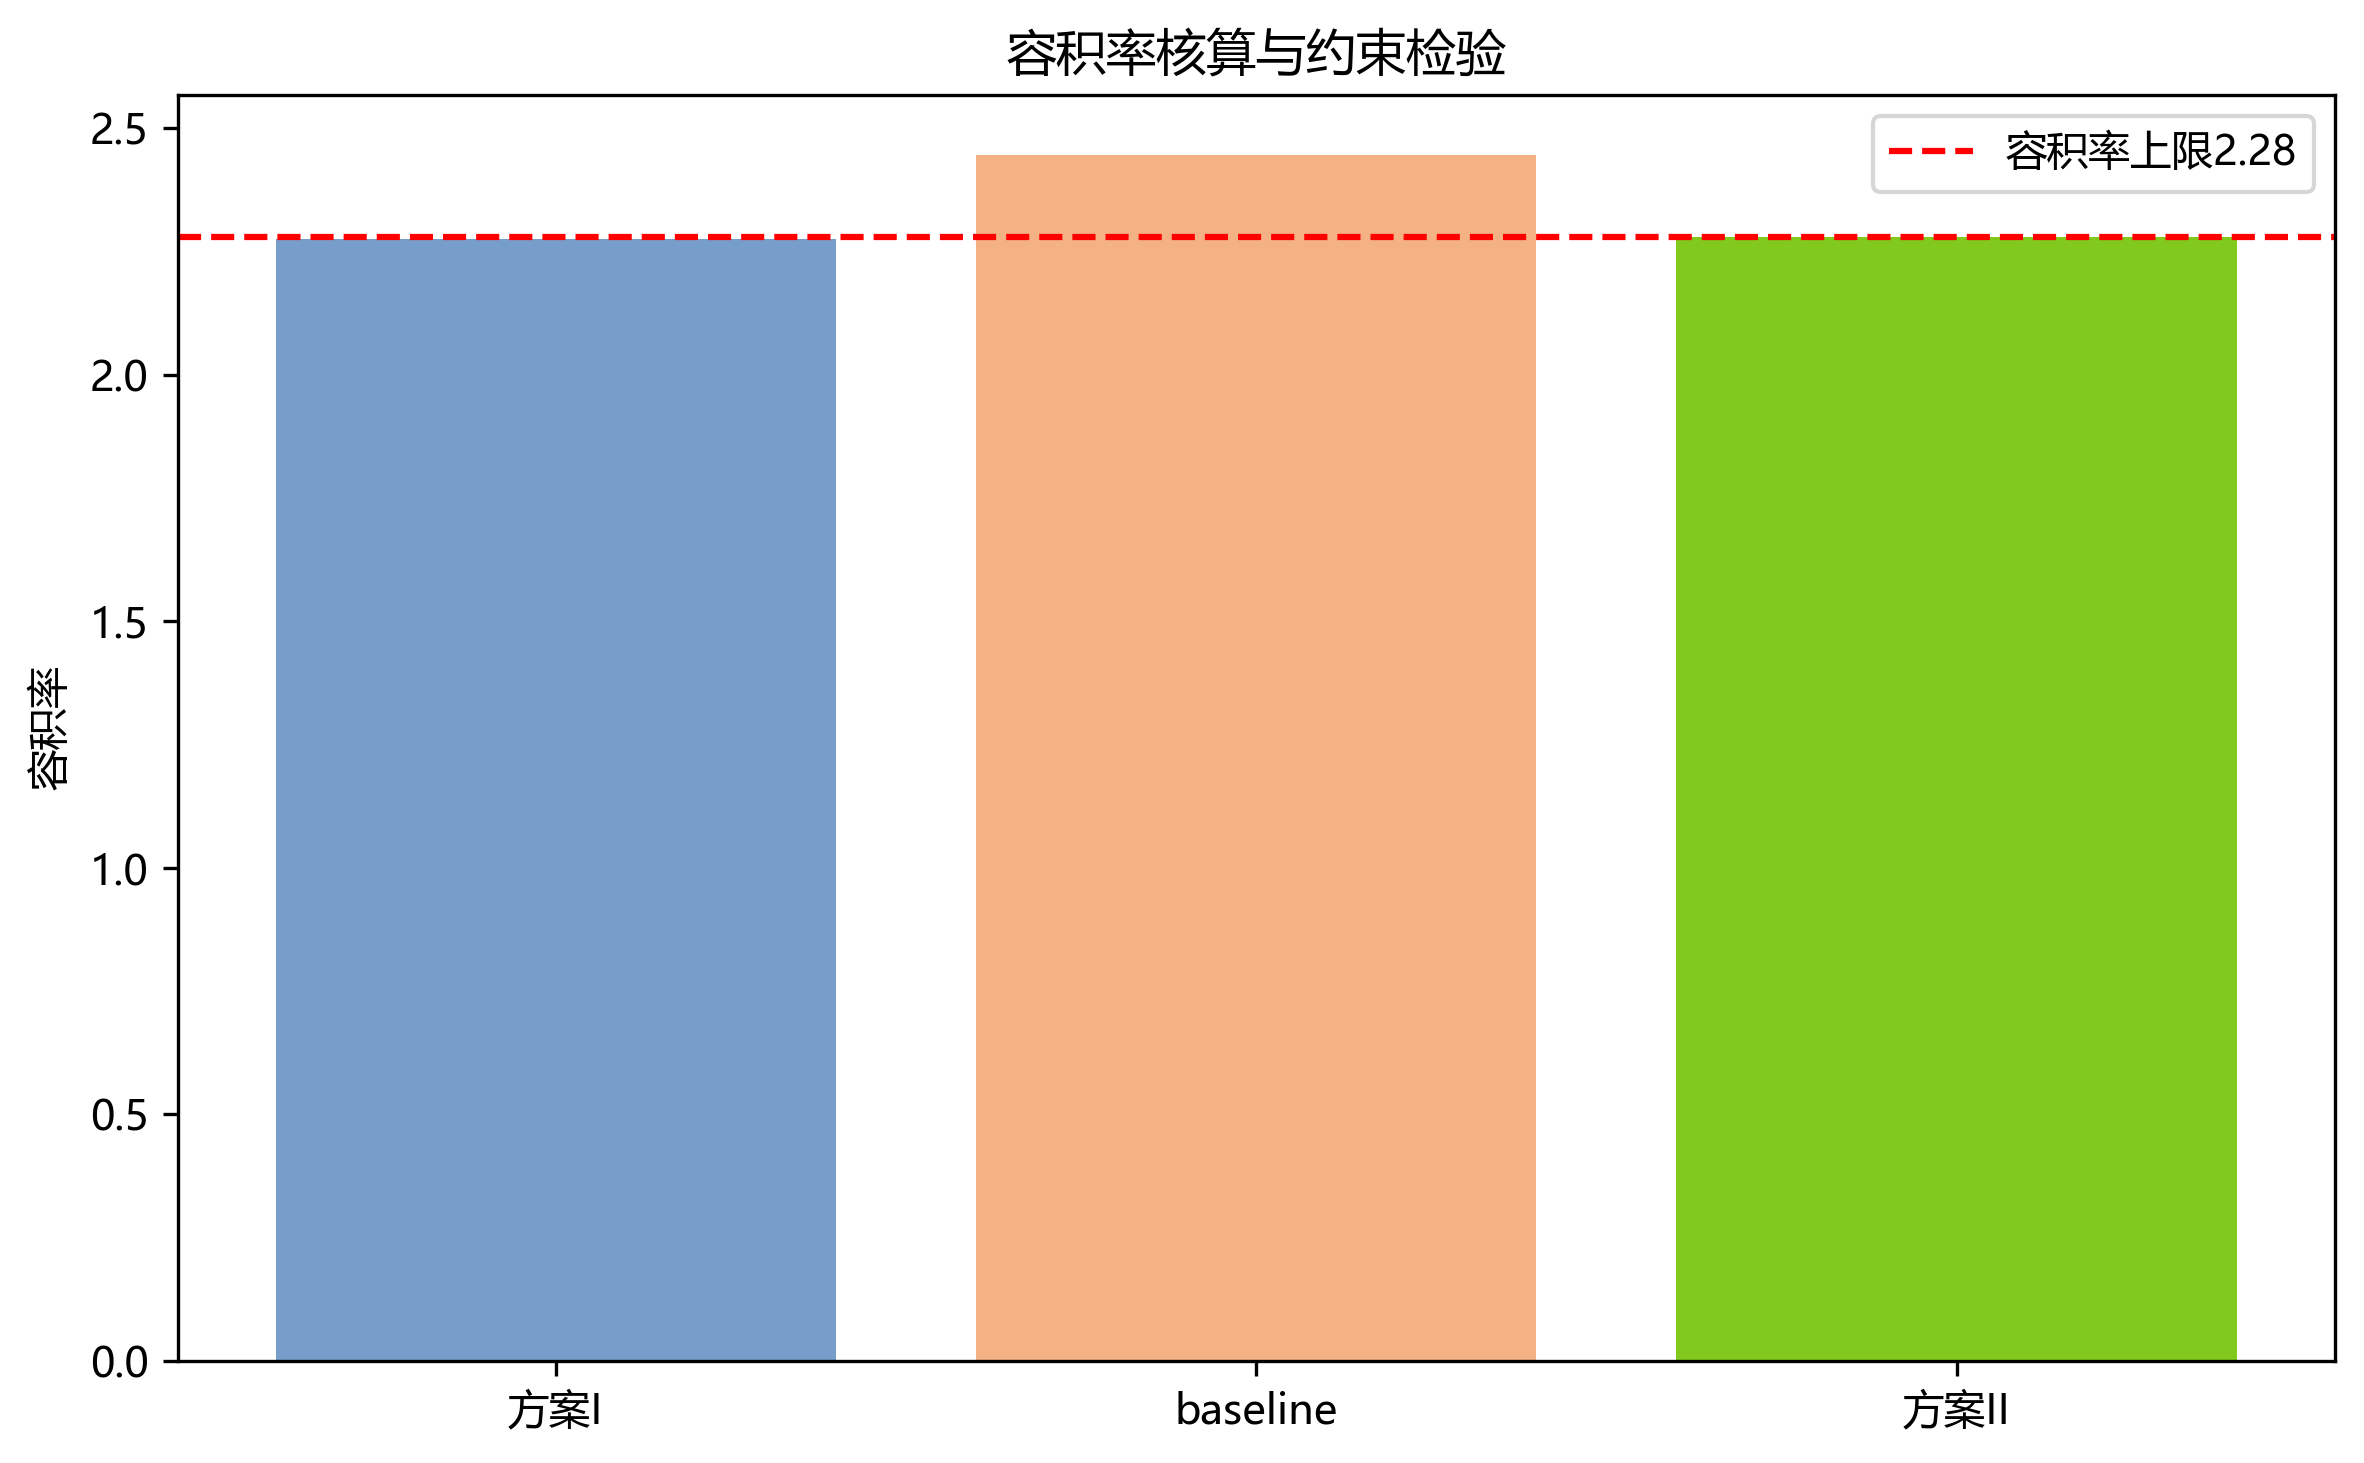
\includegraphics[width=0.72\textwidth]{问题1_容积率核算.png}\caption{容积率核算与政策上限比较}\label{fig:far}\end{figure}
图\ref{fig:far}显示，方案I和方案II均位于容积率上限以下，而偏好比例baseline超过政策上限。该结果说明单纯追求购买意愿匹配并不一定可实施，必须在优化模型中显式加入容积率约束。

\begin{table}[H]\centering\caption{方案I土地增值税分组核算}\label{tab:tax1}
\begin{tabular}{lrrrrr}\toprule
类别 & 收入/亿元 & 扣除项目/亿元 & 增值率/\% & 税率/\% & 土地增值税/亿元\\\midrule
普通住宅 & 7.5048 & 5.5161 & 36.05 & 30 & 0.5966 \\
非普通住宅 & 24.9624 & 21.5569 & 15.80 & 30 & 1.0216 \\
\bottomrule\end{tabular}\end{table}
表\ref{tab:tax1}表明，普通住宅和非普通住宅均产生正增值额。非普通住宅由于单价与面积较高，收入规模和税额贡献更大，是影响方案税后收益的关键类别。

\subsection{问题二：方案II整数规划模型}
\subsubsection{baseline模型}
为检验“满足购买意愿”的简单做法，本文将满意比例$s_i$归一化为偏好份额
\begin{equation}
w_i=\frac{s_i}{\sum_{j=1}^{11}s_j},
\end{equation}
再将总套数$N=2100$按$Nw_i$分配并投影到房型上下界。该baseline的供应结构与购买意愿非常接近，$L_1$偏差仅为0.0008，但其容积率达到2.4456，超过2.28，因而不具有可执行性。这说明问题二不能只做比例分配，必须进行带约束的优化。

\subsubsection{主模型建立}
设$x_i$为方案II第$i$种房型套数。最低和最高套数约束为
\begin{equation}
l_i\leq x_i\leq u_i,\qquad x_i\in \mathbb{Z}.
\end{equation}
为保持项目规模可比，本文令总套数与方案I一致：
\begin{equation}
\sum_{i=1}^{11}x_i=2100.
\end{equation}
容积率约束为
\begin{equation}
\sum_{i=1}^{11} a_i r_i x_i \leq 2.28L.
\end{equation}
供应结构与参筹偏好之间的偏差定义为
\begin{equation}
D(x)=\sum_{i=1}^{11}\left|\frac{x_i}{2100}-w_i\right|.
\end{equation}
为了兼顾收益和满意度，采用加权目标函数
\begin{equation}
\max \; \sum_{i=1}^{11}(a_ip_i-a_ic_i)x_i+\lambda\sum_{i=1}^{11}s_ix_i-\mu D(x),
\end{equation}
其中第一项代表税前利润，第二项代表购买意愿满意度，第三项惩罚供应偏差。绝对值项通过引入辅助变量线性化，因此可用整数线性规划求解。

\subsubsection{求解结果与解释}
方案II的房型套数如表\ref{tab:units}所示。相比方案I，方案II压缩了满意比例较低或单位收益较弱的房型1、房型3、房型9，同时增加了房型2、房型6、房型7、房型10和房型11。该结构既保留了高满意度房型，又通过非计容或较高收益房型提高财务表现。

\begin{table}[H]\centering\caption{方案II各房型建设套数}\label{tab:units}
\begin{tabular}{lr}\toprule
房型 & 方案II套数\\\midrule
房型1 & 50 \\
房型2 & 354 \\
房型3 & 50 \\
房型4 & 150 \\
房型5 & 100 \\
房型6 & 349 \\
房型7 & 450 \\
房型8 & 100 \\
房型9 & 50 \\
房型10 & 197 \\
房型11 & 250 \\
\bottomrule\end{tabular}\end{table}

\begin{figure}[H]\centering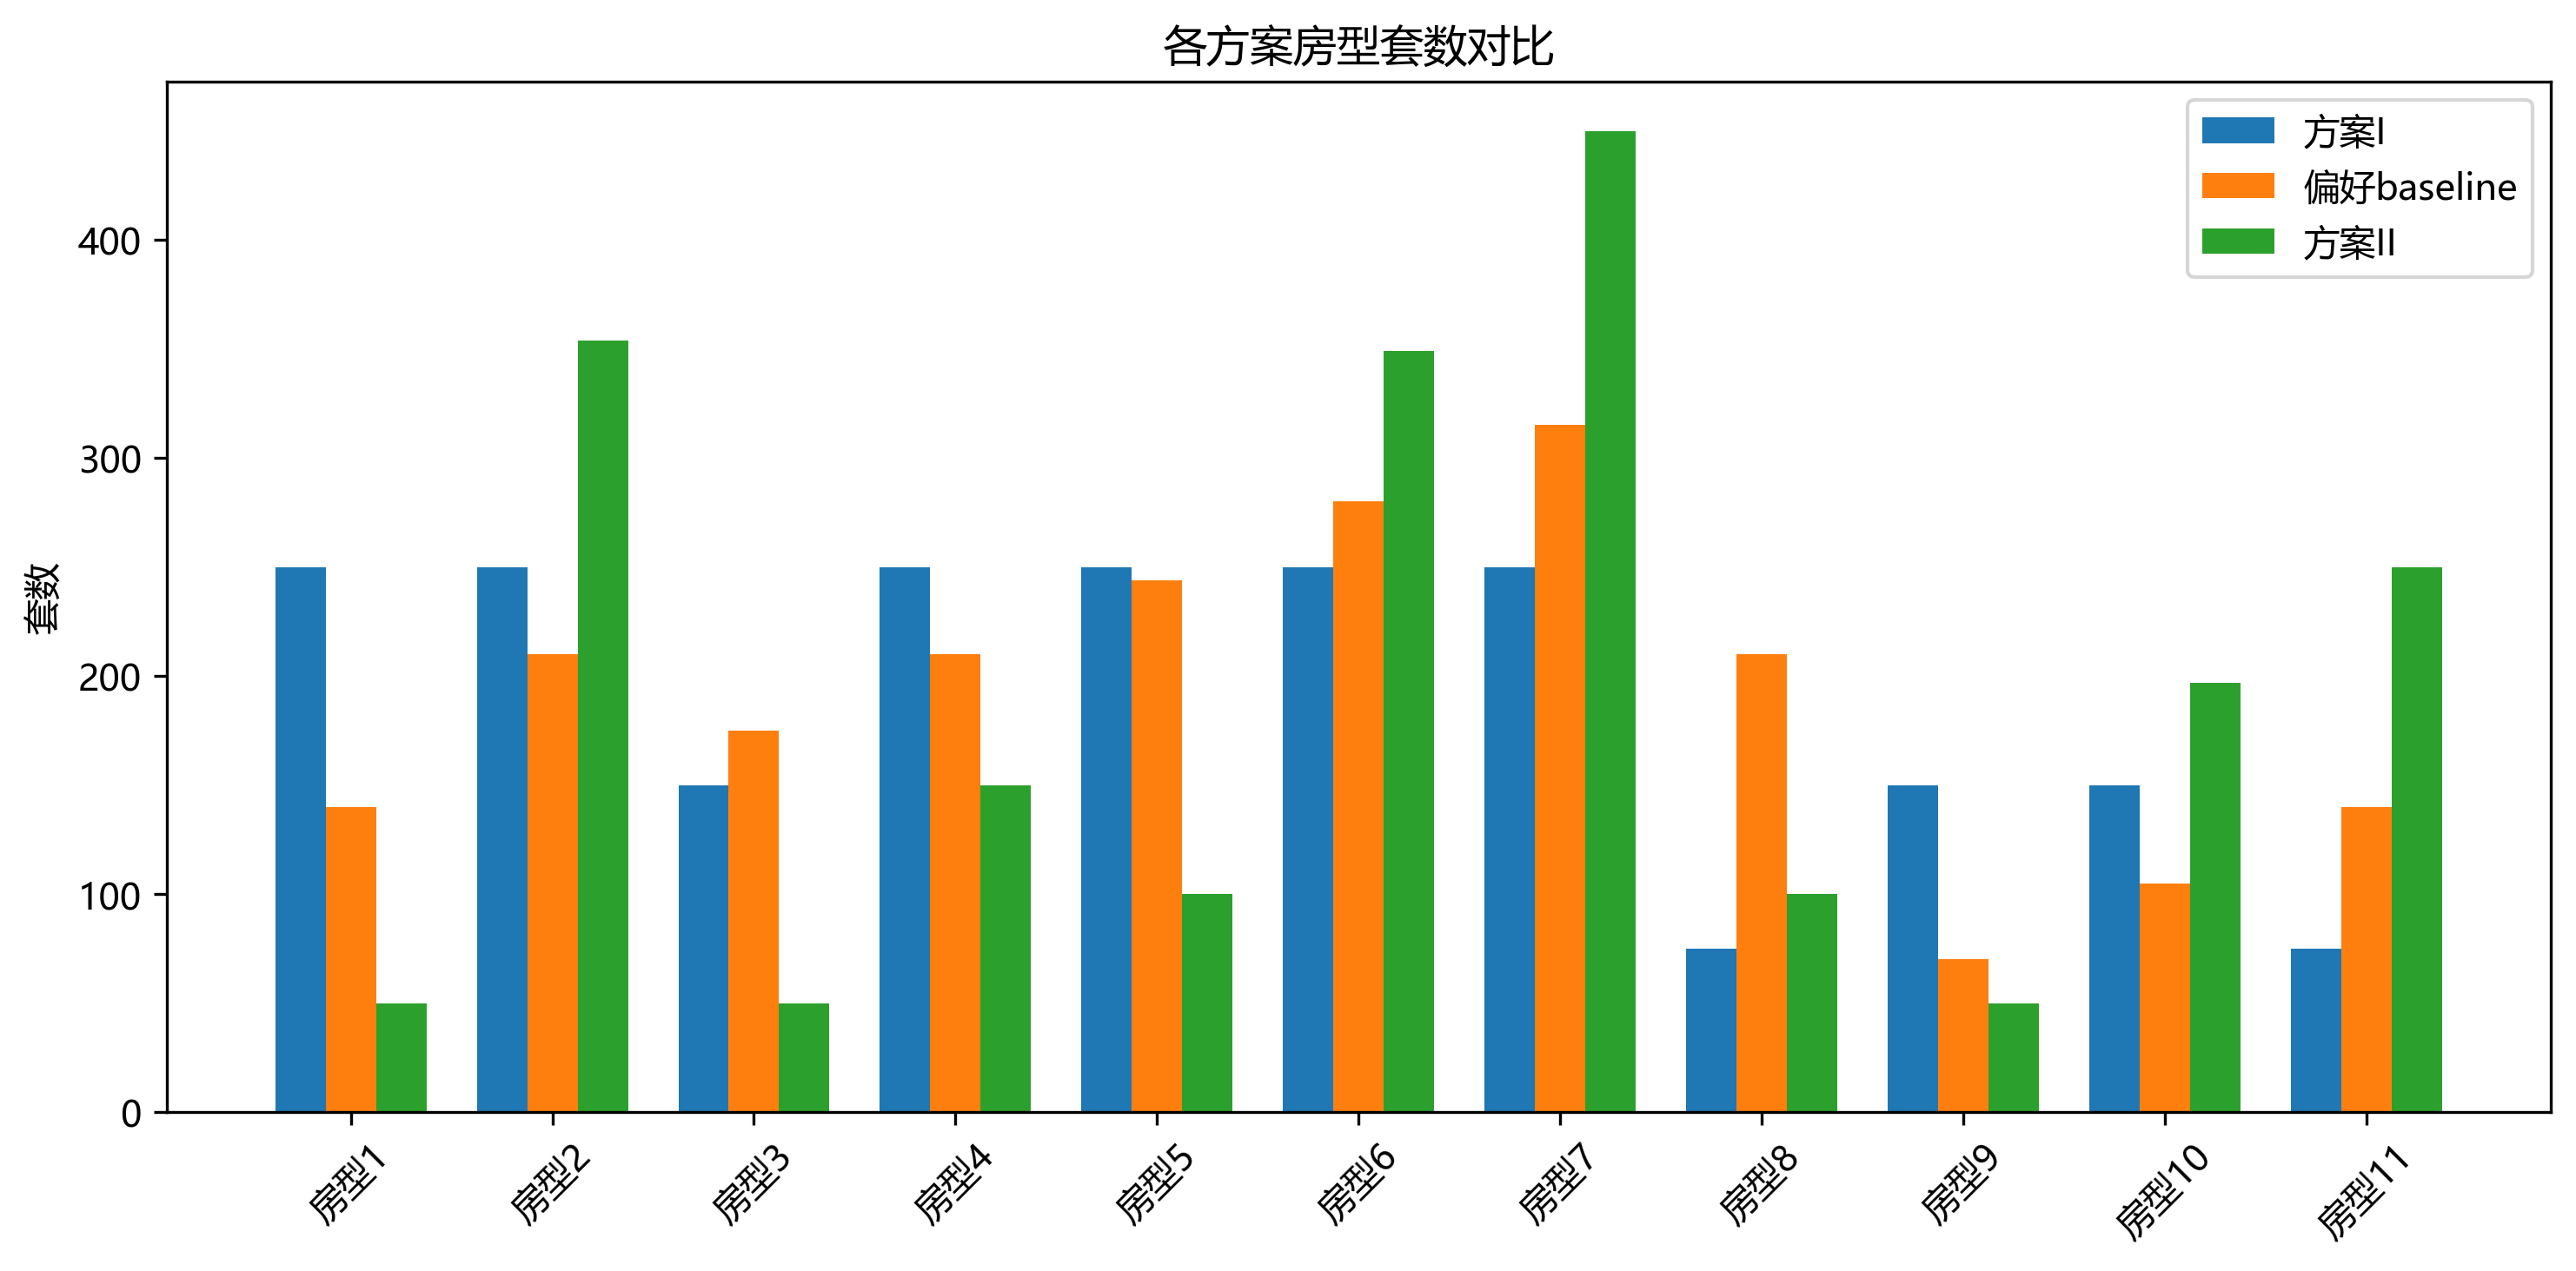
\includegraphics[width=0.86\textwidth]{问题2_房型套数对比.png}\caption{方案I、baseline与方案II房型套数对比}\label{fig:units}\end{figure}
图\ref{fig:units}直观展示了三种方案的结构差异。baseline几乎完全跟随满意比例，因此在高满意房型上大量增加套数，却导致容积率超限；方案II则在高满意、高收益和不计容房型之间折中，使得方案可执行。

\begin{figure}[H]\centering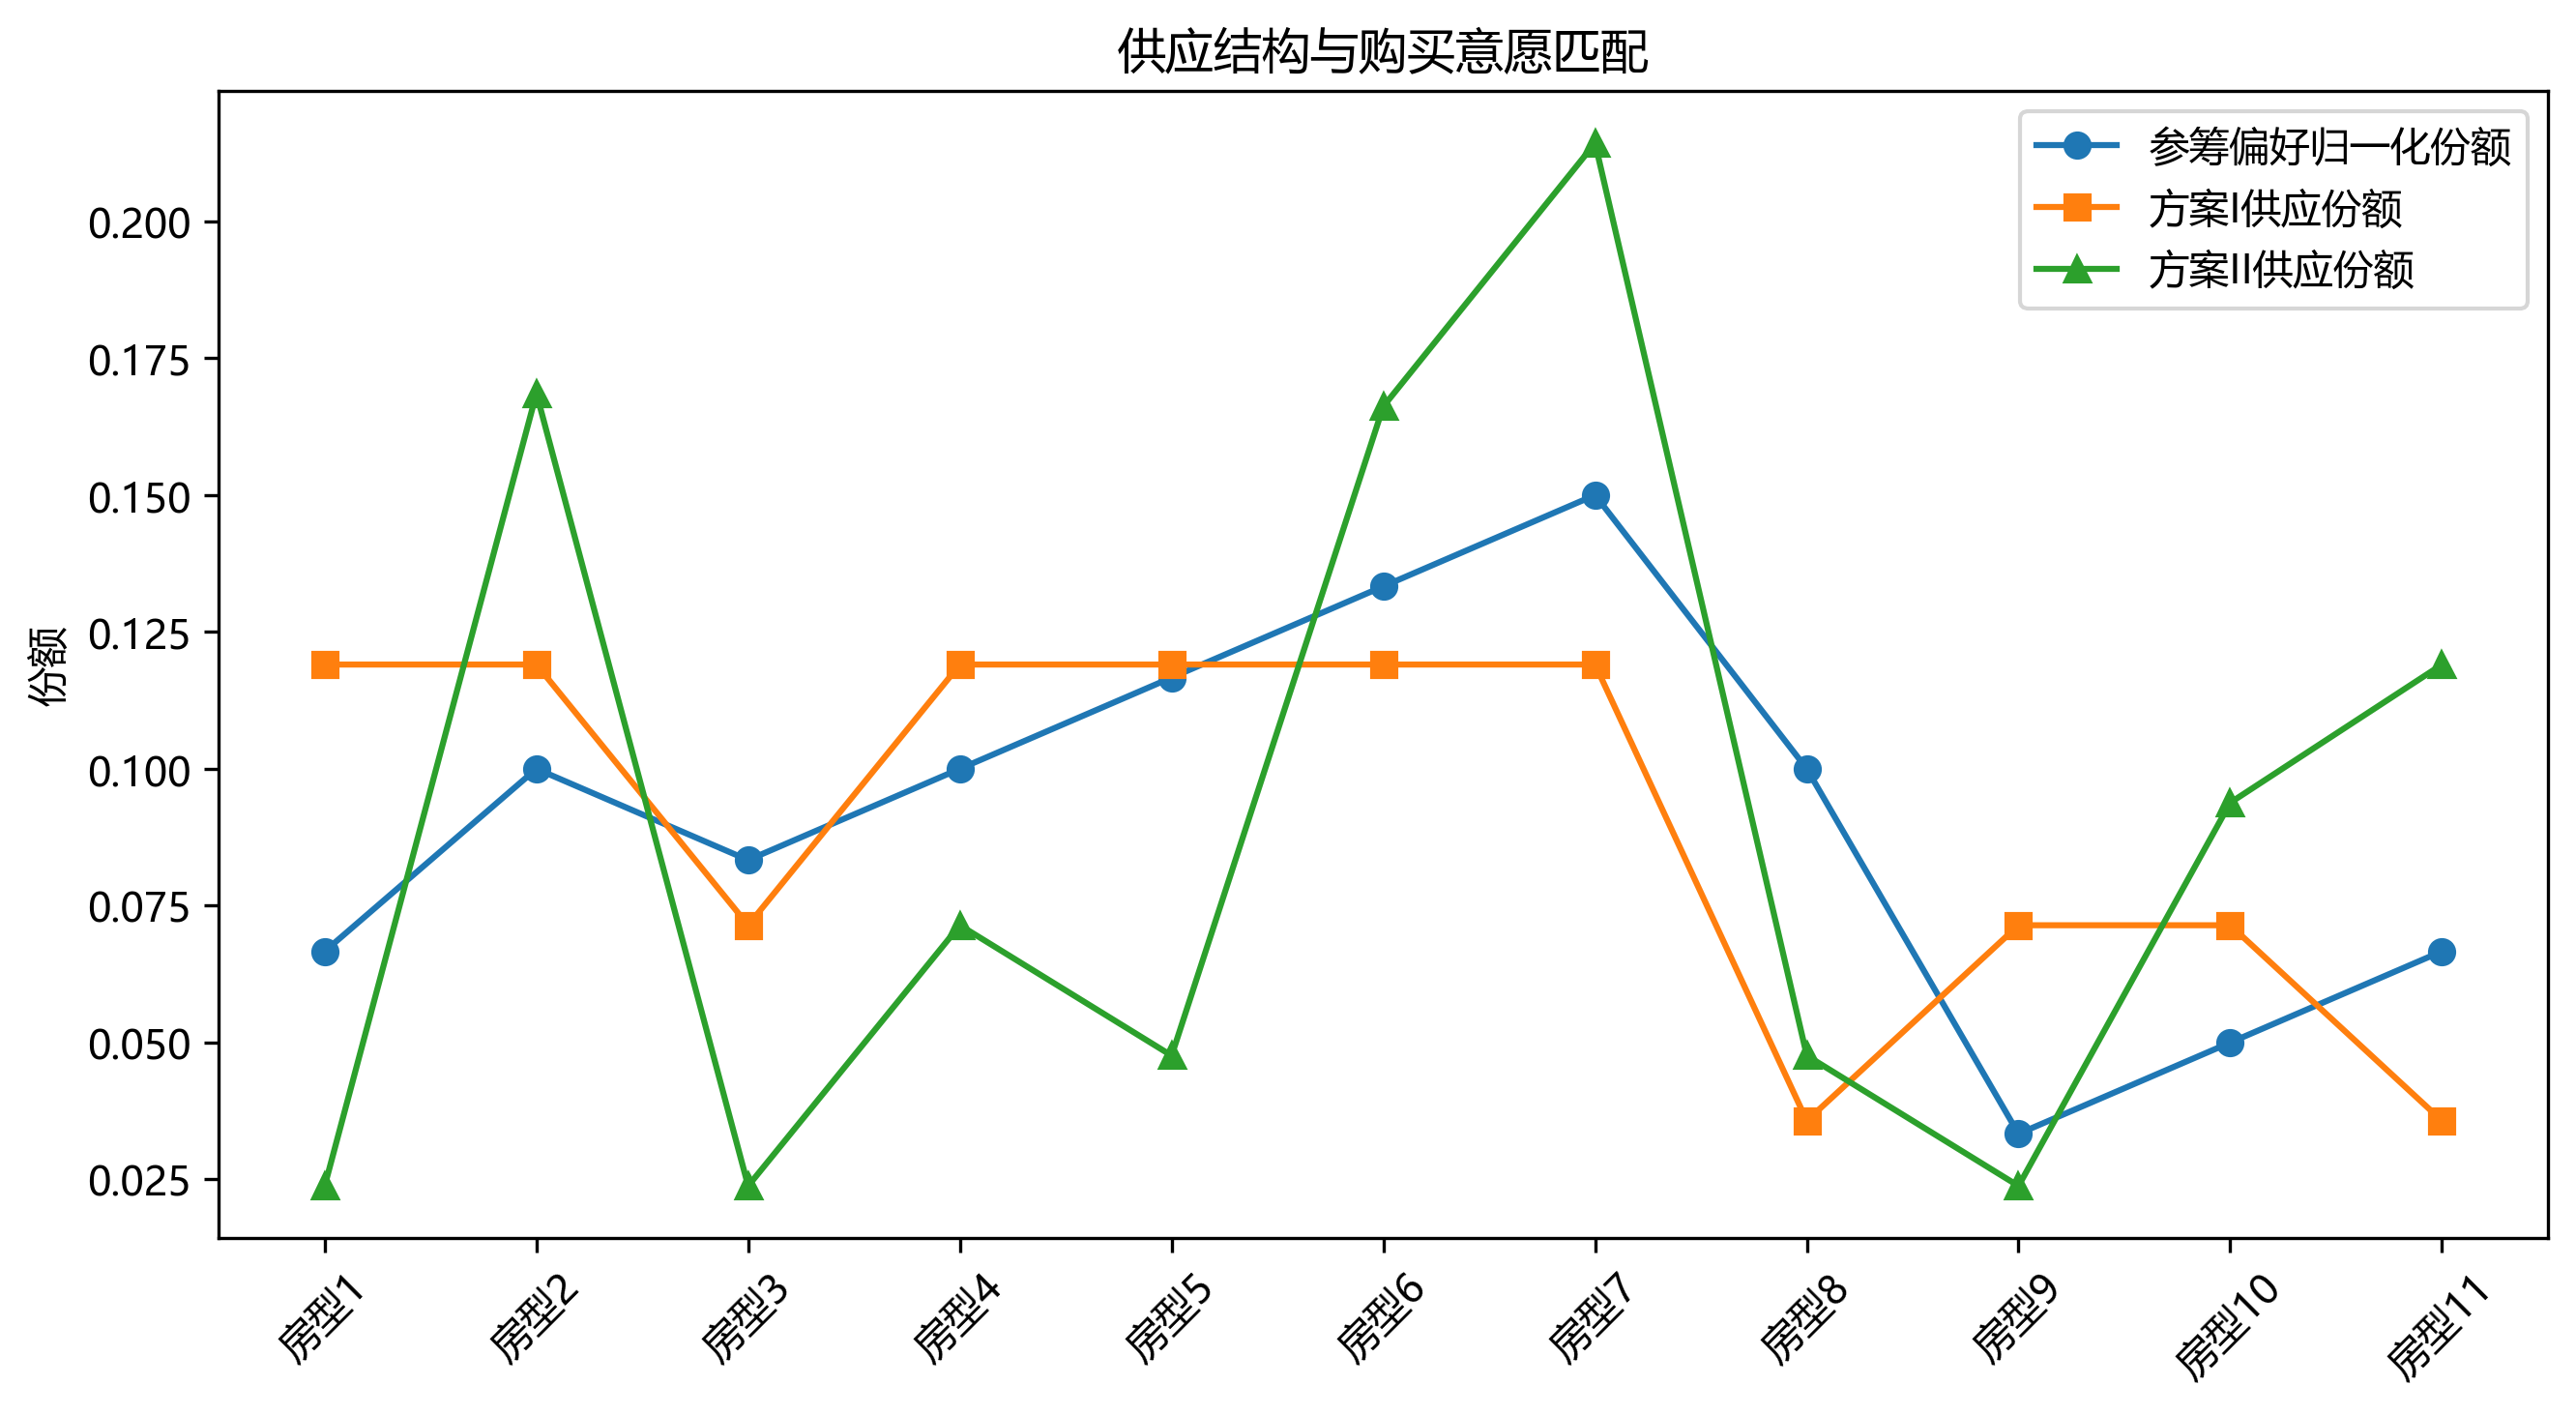
\includegraphics[width=0.86\textwidth]{问题2_意愿匹配曲线.png}\caption{供应结构与参筹购买意愿匹配曲线}\label{fig:match}\end{figure}
图\ref{fig:match}显示，方案II不是简单复制偏好曲线，而是在政策约束下提高整体满意得分。其加权满意得分为0.6337，高于方案I的0.5833。虽然$L_1$偏差大于baseline，但baseline不可行，因此方案II在可行性和满意度之间取得了更合理平衡。

\begin{table}[H]\centering\caption{方案II土地增值税分组核算}\label{tab:tax2}
\begin{tabular}{lrrrrr}\toprule
类别 & 收入/亿元 & 扣除项目/亿元 & 增值率/\% & 税率/\% & 土地增值税/亿元\\\midrule
普通住宅 & 5.2074 & 4.1638 & 25.06 & 30 & 0.3131 \\
非普通住宅 & 29.3399 & 23.8304 & 23.12 & 30 & 1.6529 \\
\bottomrule\end{tabular}\end{table}
表\ref{tab:tax2}给出了方案II的税负结构。由于方案II增加了部分高收入房型，销售收入提高到34.5473亿元；土地增值税也相应提高到1.9659亿元。但税后净利润仍达到8.7956亿元，高于方案I。

\subsection{问题三：投资回报率与调整分析}
\subsubsection{成功性判断}
方案II的总成本为25.7517亿元，净利润为8.7956亿元，投资回报率为34.16\%。由于34.16\%大于25\%，因此在附件给定价格、成本和税收口径下，方案II可以被成功执行。

\begin{figure}[H]\centering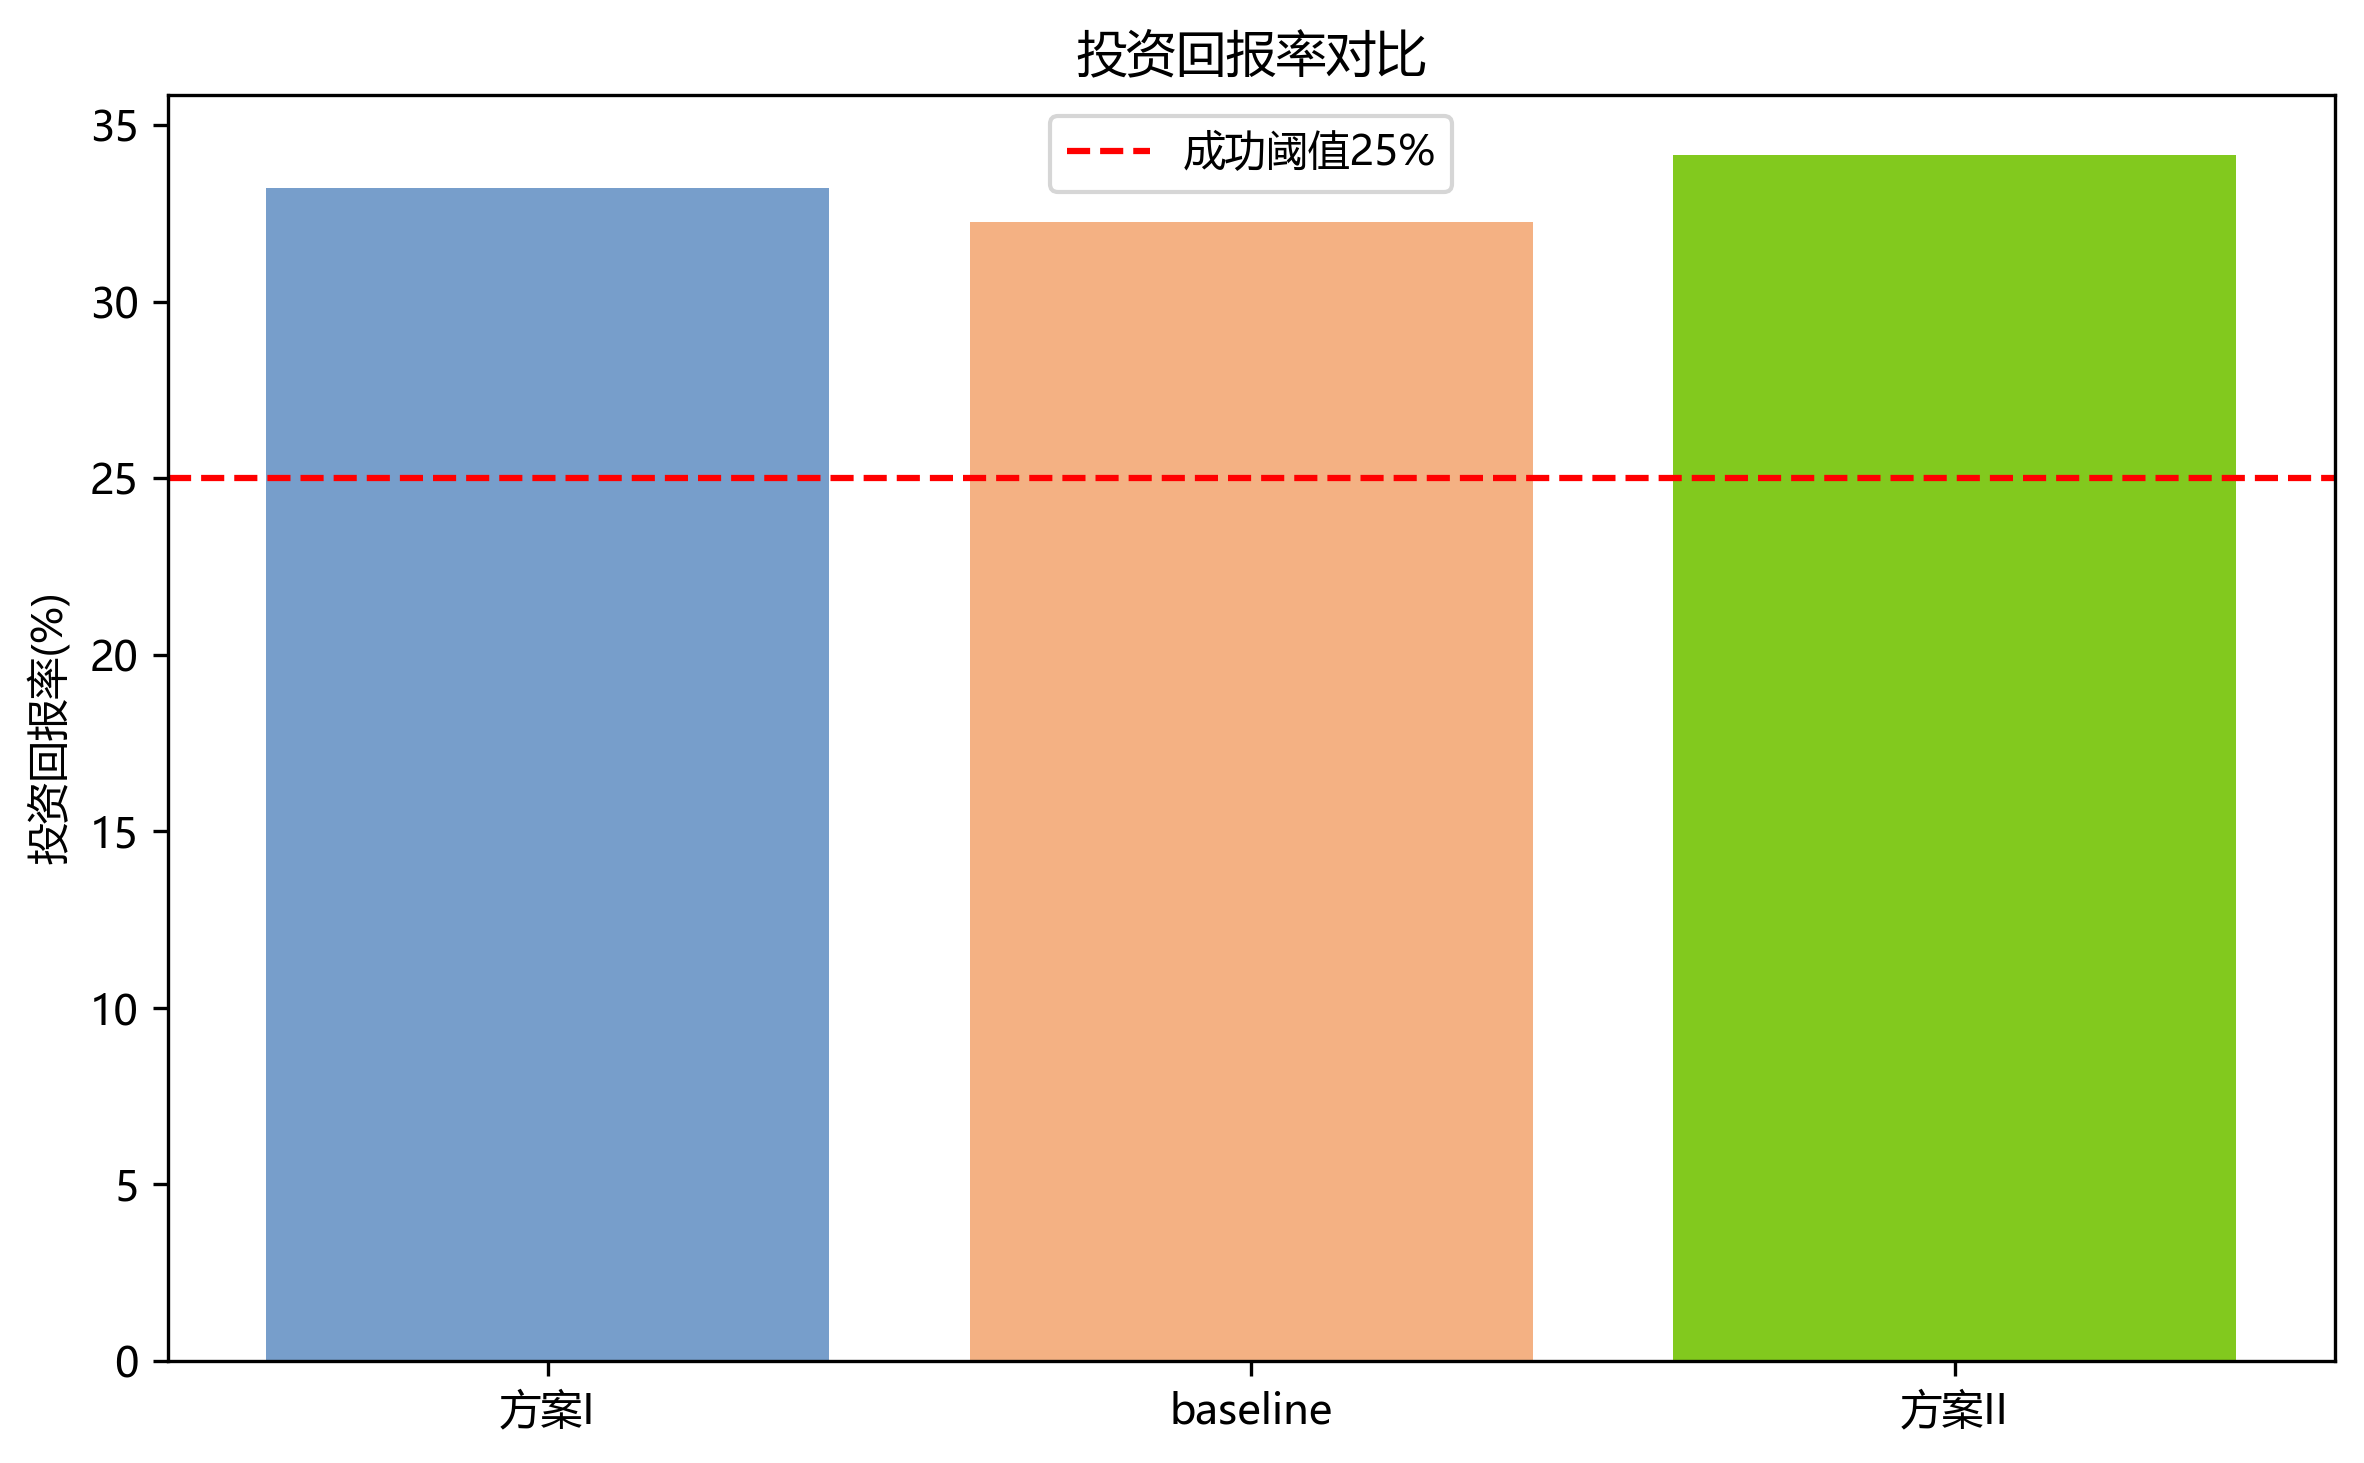
\includegraphics[width=0.72\textwidth]{问题3_投资回报率对比.png}\caption{方案投资回报率与25\%成功阈值比较}\label{fig:roi}\end{figure}
图\ref{fig:roi}显示，方案I、baseline和方案II的ROI均高于25\%，但baseline违反容积率约束，不能作为正式方案。方案II在可行约束下ROI最高，因此是本文推荐的实施方案。

\subsubsection{敏感性分析}
为检验结论稳健性，本文分别设置售价系数$\alpha$和建安成本系数$\beta$，重新计算方案II的税后ROI：
\begin{align}
p_i'&=\alpha p_i,\\
c_i'&=\beta c_i.
\end{align}
扰动范围取0.92--1.12和0.88--1.08。敏感性结果如图\ref{fig:sens}所示。

\begin{figure}[H]\centering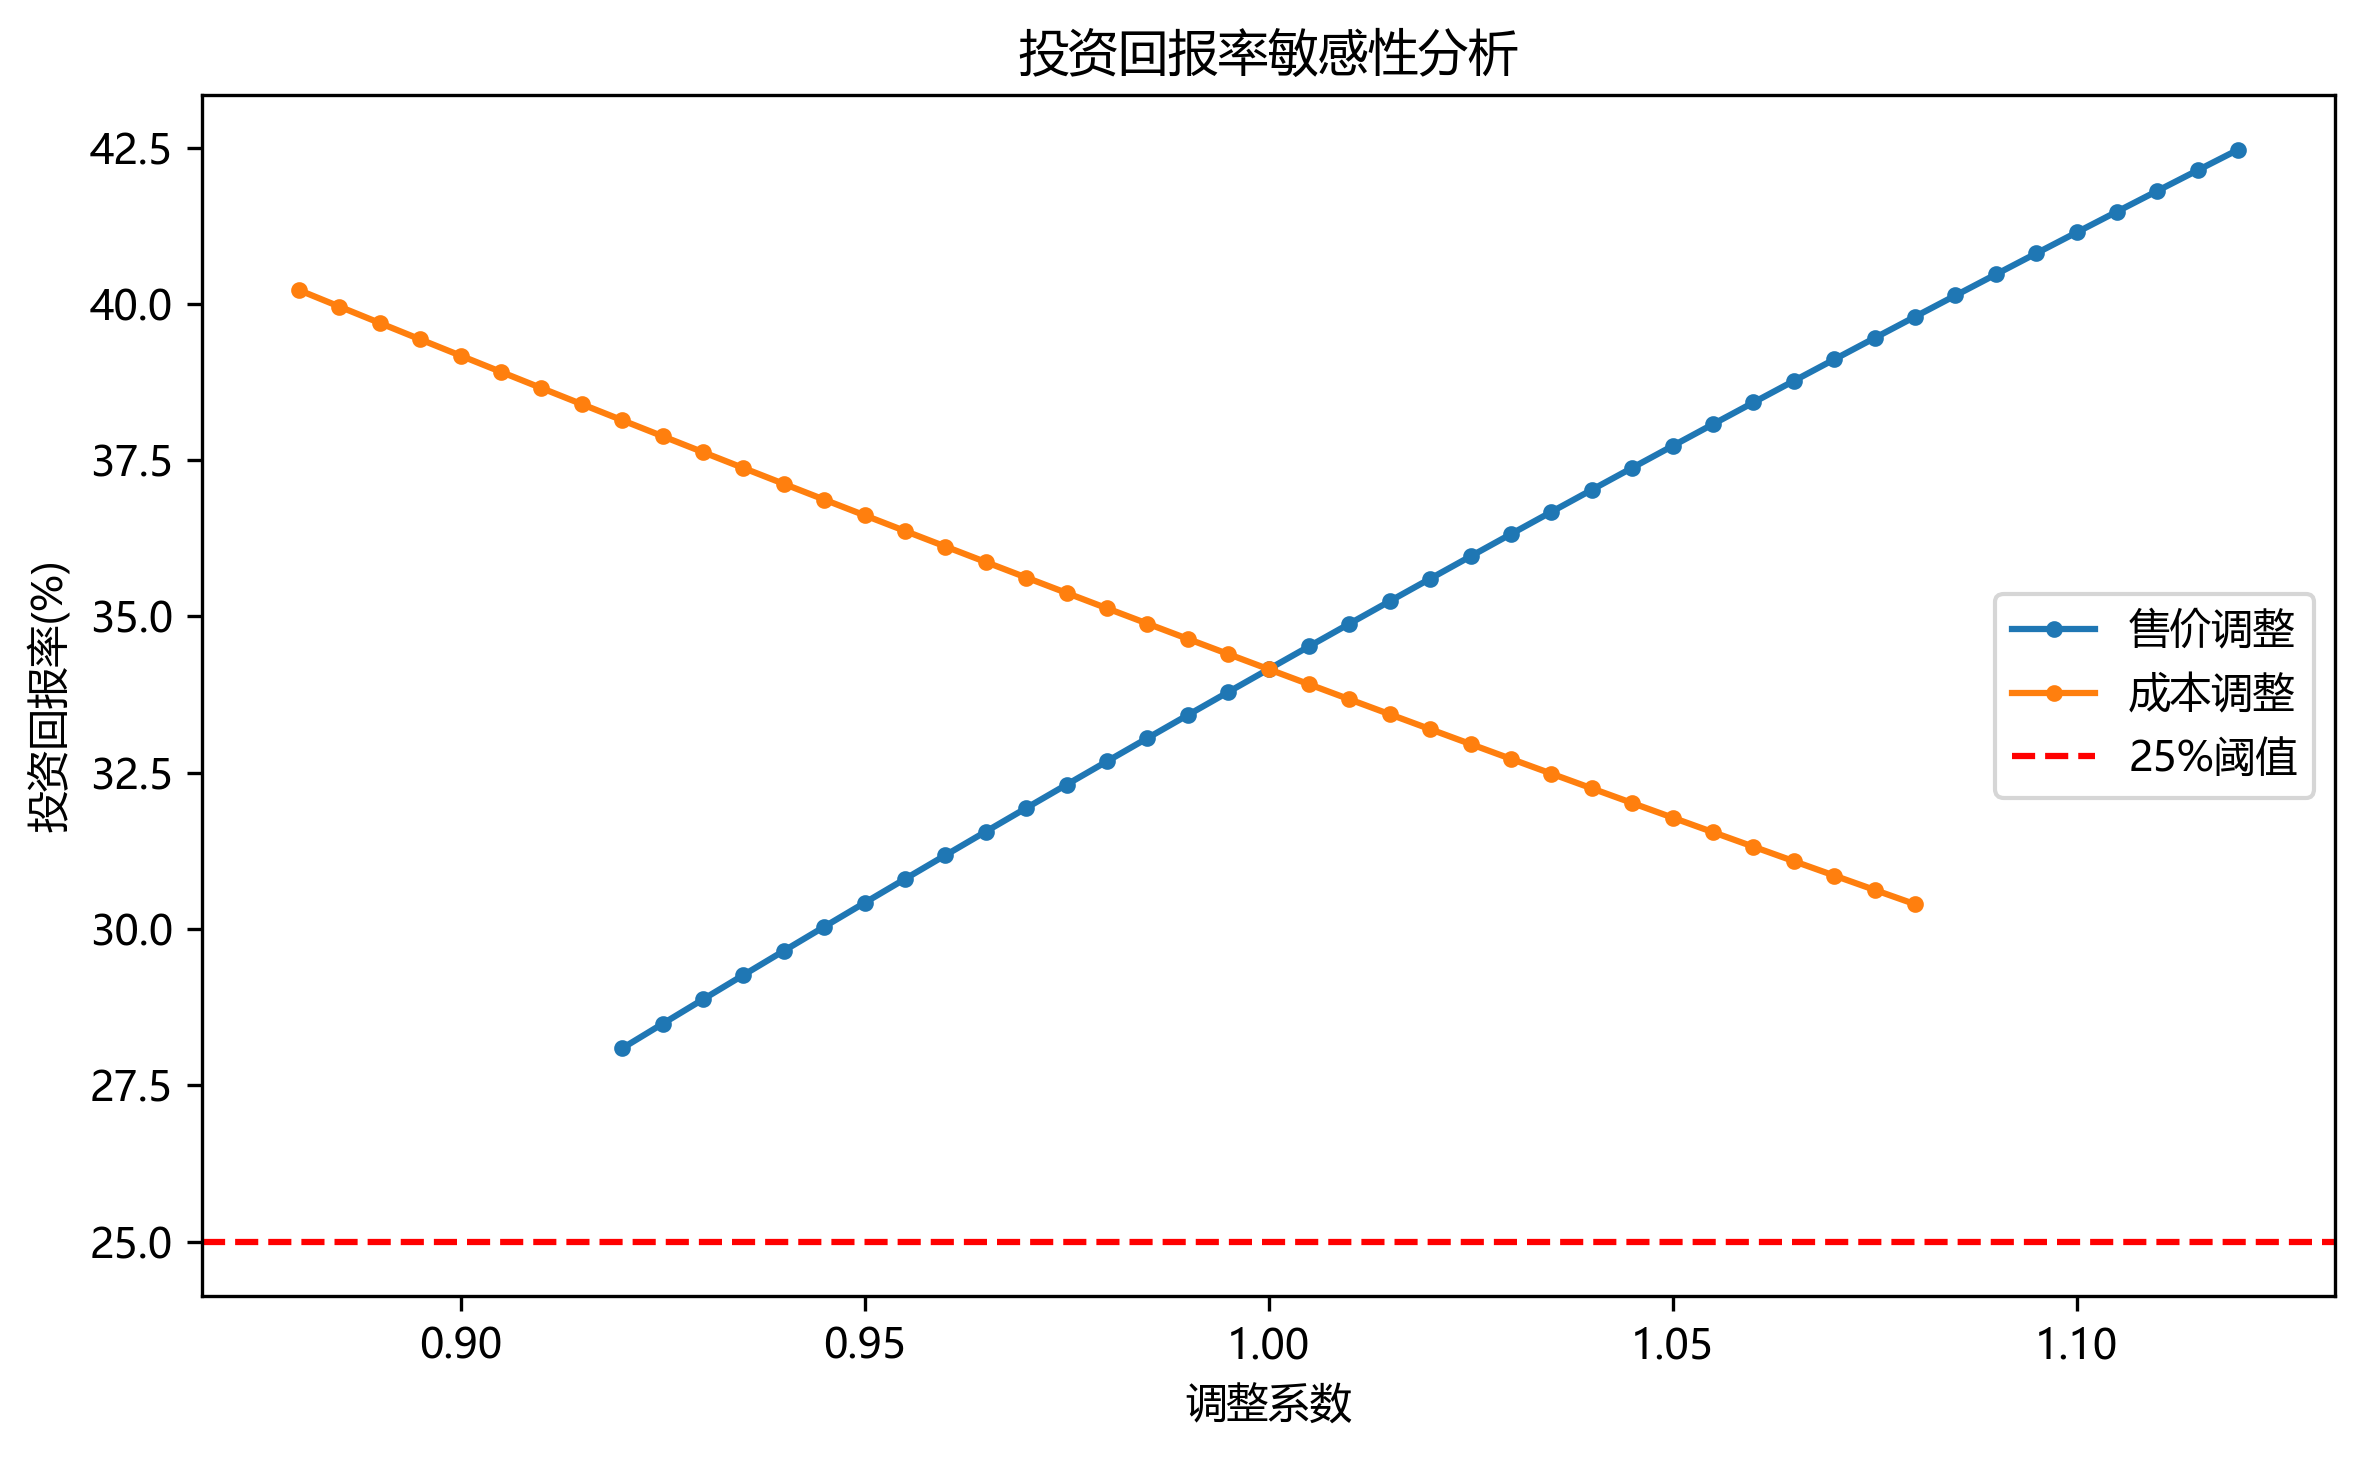
\includegraphics[width=0.78\textwidth]{问题3_ROI敏感性分析.png}\caption{方案II投资回报率敏感性分析}\label{fig:sens}\end{figure}
从图\ref{fig:sens}可以看出，售价上升会显著提高ROI，建安成本上升会降低ROI，但在本文设定的扰动范围内曲线整体仍处于25\%阈值上方。因此方案II不只是单点达标，而是在一定市场波动下仍有安全裕度。若未来出现更大幅度的价格下降或成本上升，可优先采取三类调整：一是适度提高高满意高收益房型售价；二是压缩单位开发成本较高且满意度一般的房型；三是在容积率允许范围内增加高收益不计容或低计容压力房型。

\section{模型检验、对比与稳健性}
\subsection{约束检验}
方案II满足所有房型最低和最高套数约束，且总套数保持为2100套。容积率为2.2799，与上限2.28的差距为0.0001。由于模型求解时已将计容面积作为线性约束，约束残差为非正值，说明优化方案具备政策可行性。

\subsection{baseline对比}
baseline的优势是购买意愿匹配度高，$L_1$偏差仅0.0008；但其容积率为2.4456，超出政策上限，因而不可执行。方案II牺牲部分结构匹配，换取容积率可行、税后利润提高和ROI提高。相较方案I，方案II净利润提高0.6967亿元，ROI提高0.92个百分点，加权满意得分提高0.0503。

\subsection{税负核算复核}
本文将“其他”类别按普通住宅和非普通住宅建筑面积比例分摊，避免忽略特殊类别收入与成本。土地增值税采用分组超率累进方式计算，税率与增值率区间一一对应。所有税额均由代码自动生成，并写入\texttt{tables/土地增值税分组核算.csv}。论文表格中的税额与\texttt{results/frozen\_numbers.json}一致。

\subsection{稳健性讨论}
售价和成本敏感性分析表明，方案II在一定范围内仍高于25\%阈值。对优化模型而言，主要不确定性来自满意比例样本是否能代表全部参筹者，以及未来市场价格是否偏离附件售价。若后续获得更大规模调查数据，可将满意比例替换为分层抽样需求份额，并将售价设为随机变量进行蒙特卡洛模拟。

\section{模型评价、改进与推广}
\subsection{模型优点}
第一，本文模型链完整，从题目附件直接生成核算结果、优化方案和论文图表，所有关键数字可追溯到冻结文件。第二，方案II使用整数规划，能够同时处理套数上下界、容积率和总套数等硬约束，避免比例分配造成不可行方案。第三，土地增值税按普通住宅和非普通住宅分组计算，并处理“其他”类别分摊，较简单税率模型更符合政策口径。第四，模型不仅给出最终方案，还通过baseline对比和敏感性分析说明方案的可行性与稳健性。

\subsection{模型局限}
第一，附件中满意比例只有“满意/不满意”二元结果，不能完整描述购房者价格敏感性、户型替代关系和支付能力。第二，开发费用和加计扣除采用政策常用比例估算，实际清算时可能受财务凭证、利息支出和地方执行细则影响。第三，模型假设方案II售价和成本与方案I相同，未考虑批量建设、楼栋布局或市场供需变化对价格和成本的反馈。

\subsection{改进方向与推广}
后续可从三方面改进：一是引入更细致的需求调查数据，建立离散选择模型或Logit需求模型；二是将税务核算与现金流时间序列结合，计算净现值和内部收益率；三是将建筑布局、楼栋层数和配套设施纳入多目标规划。本文方法可推广到保障房配比、商业住宅户型组合设计、产业园区功能面积配置等需要在政策约束、用户偏好和投资收益之间平衡的问题。

\section{结论}
本文完成了2015D众筹筑屋规划方案的全流程建模。主要结论如下：
\begin{enumerate}
\item 方案I总套数为2100套，容积率2.2752，满足2.28上限；销售收入32.4672亿元，土地增值税1.6183亿元，净利润8.0989亿元，ROI为33.24\%。
\item 偏好比例baseline虽能很好匹配购买意愿，但容积率为2.4456，不可执行。方案II通过整数规划得到可行套数配置：房型150套, 房型2354套, 房型350套, 房型4150套, 房型5100套, 房型6349套, 房型7450套, 房型8100套, 房型950套, 房型10197套, 房型11250套。
\item 方案II容积率为2.2799，满足政策约束；销售收入34.5473亿元，净利润8.7956亿元，ROI为34.16\%，高于25\%项目成功阈值，推荐执行。
\item 敏感性分析显示，方案II在一定售价和成本扰动范围内仍保持较高ROI，说明方案具有较好的稳健性。若市场环境恶化，可优先调整高满意高收益房型比例和成本控制策略。
\end{enumerate}

\section*{参考文献}
\addcontentsline{toc}{section}{参考文献}
\begin{enumerate}[label={[\arabic*]},leftmargin=2.5em]
\item 国务院. 中华人民共和国土地增值税暂行条例[Z]. 1993.
\item 财政部, 国家税务总局. 关于土地增值税若干问题的通知[Z]. 2006.
\item 财政部, 国家税务总局. 土地增值税清算管理规程[S]. 2009.
\item 胡运权. 运筹学教程[M]. 北京: 清华大学出版社, 2018.
\item 姜启源, 谢金星, 叶俊. 数学模型[M]. 北京: 高等教育出版社, 2018.
\item SciPy Developers. scipy.optimize.milp documentation[EB/OL]. 2026.
\end{enumerate}

\appendix
\section{支撑材料说明}
本次建模支撑材料位于题目目录下的\texttt{支撑材料/}。其中\texttt{代码/2015D\_complete\_solution.py}为完整可运行代码；\texttt{tables/}保存输入数据、方案核算、候选比较和敏感性分析表；\texttt{图表/}保存论文所用PNG图；\texttt{results/frozen\_numbers.json}保存冻结数字；\texttt{contracts/}保存题意、模型路线、结果、指标和结论契约。

\section{代码复现方式}
在Windows bash环境中运行：
\begin{verbatim}
cd <LOCAL_MATH_MODELING_TEST_ROOT>/2015年赛题/2015D/支撑材料
python 代码/2015D_complete_solution.py
cd 论文
xelatex -interaction=nonstopmode 论文.tex
xelatex -interaction=nonstopmode 论文.tex
xelatex -interaction=nonstopmode 论文.tex
\end{verbatim}

\end{document}
